\subsubsection{Client}

Giao diện của client được viết trong hàm \texttt{void menu()} với 3 chức năng chính:
\begin{itemize}
    \item \textbf{Start:} Khởi tạo kết nối với server, bắt đầu đọc email từ Gmail và giao tiếp với server.
    \item \textbf{Add Gmail:} Thêm tài khoản Gmail Admin để nhận lệnh điều khiển từ Gmail này.
    \item \textbf{Instruction:} Hiển thị hướng dẫn sử dụng và các lệnh điều khiển.
\end{itemize}

Dưới đây là một số hình ảnh minh họa cho giao diện của client:
\begin{figure}[H]
    \centering
    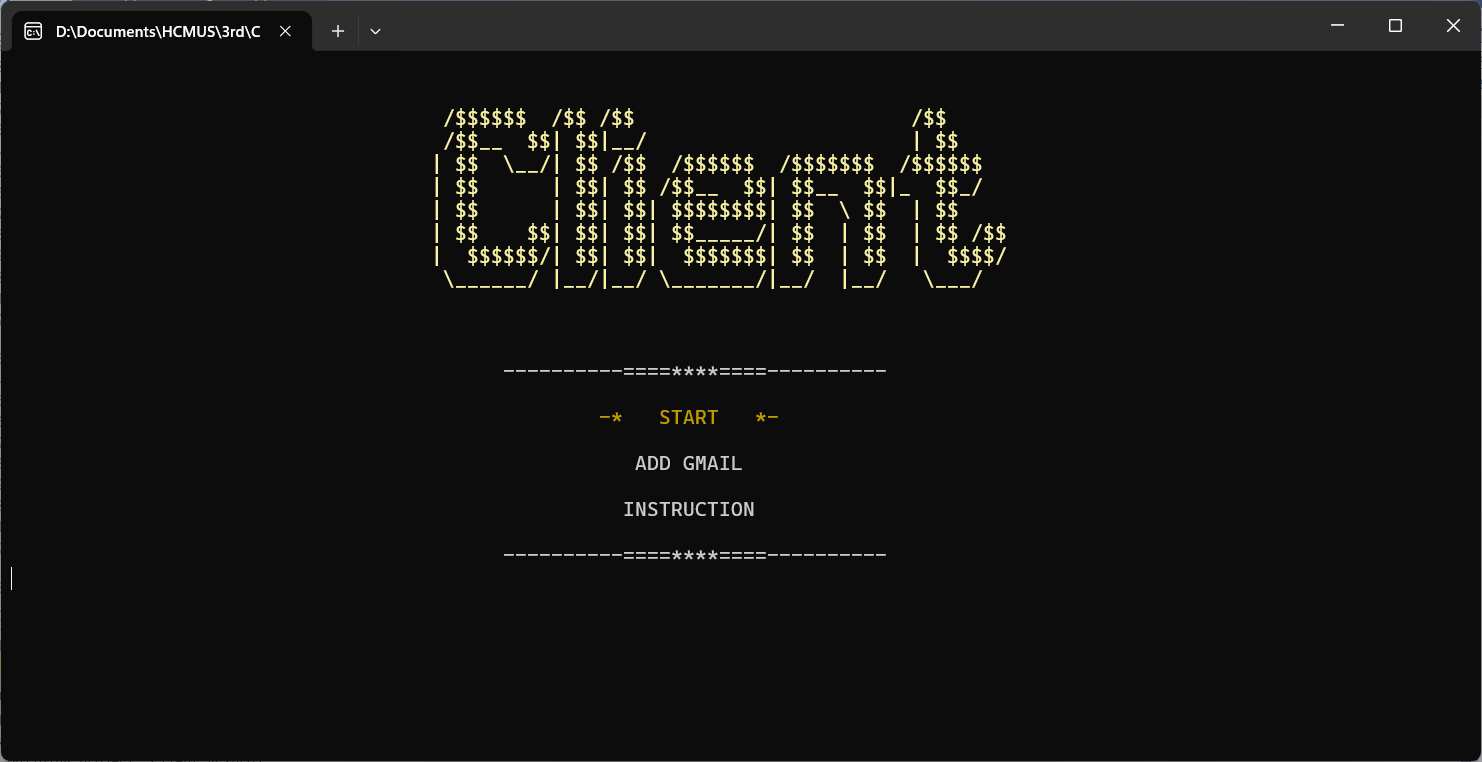
\includegraphics[width=0.7\textwidth]{img/client.png}
    \caption{Giao diện của client}
\end{figure}

\begin{figure}
    \centering
    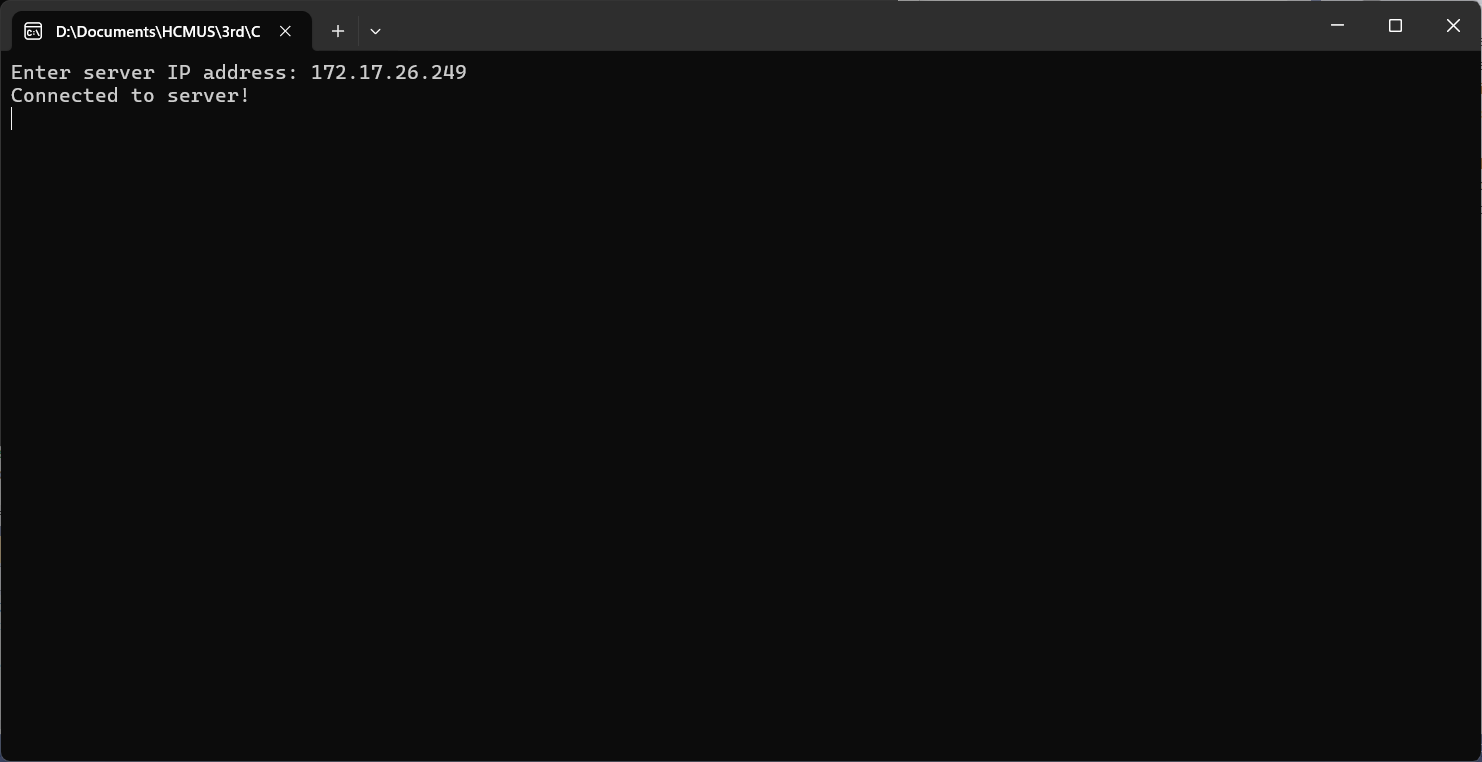
\includegraphics[width=0.7\textwidth]{img/start.png}
    \caption{Bắt đầu kết nối với server}
\end{figure}

\begin{figure}[H]
    \centering
    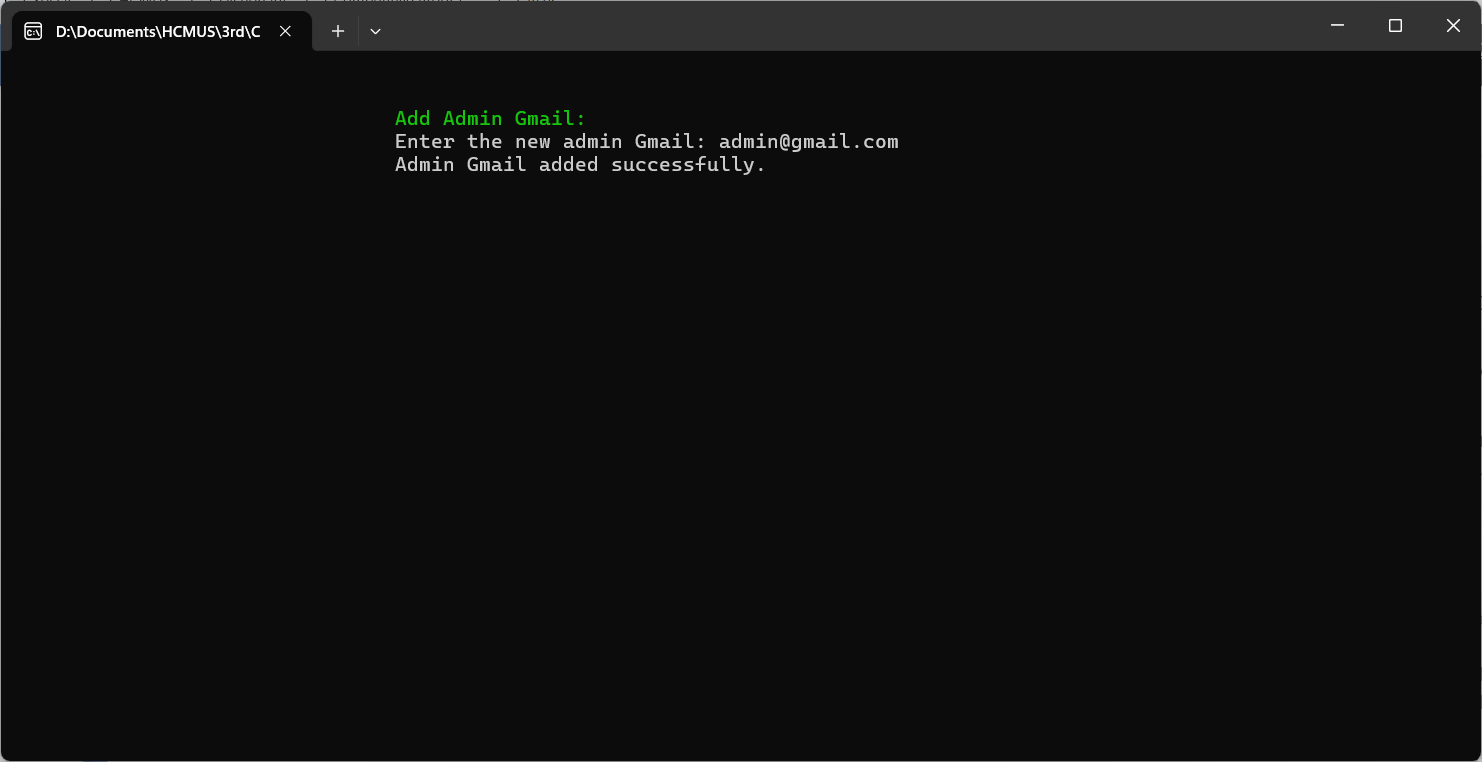
\includegraphics[width=0.7\textwidth]{img/add_gmail.png}
    \caption{Thêm tài khoản Gmail Admin}
\end{figure}

\begin{figure}[H]
    \centering
    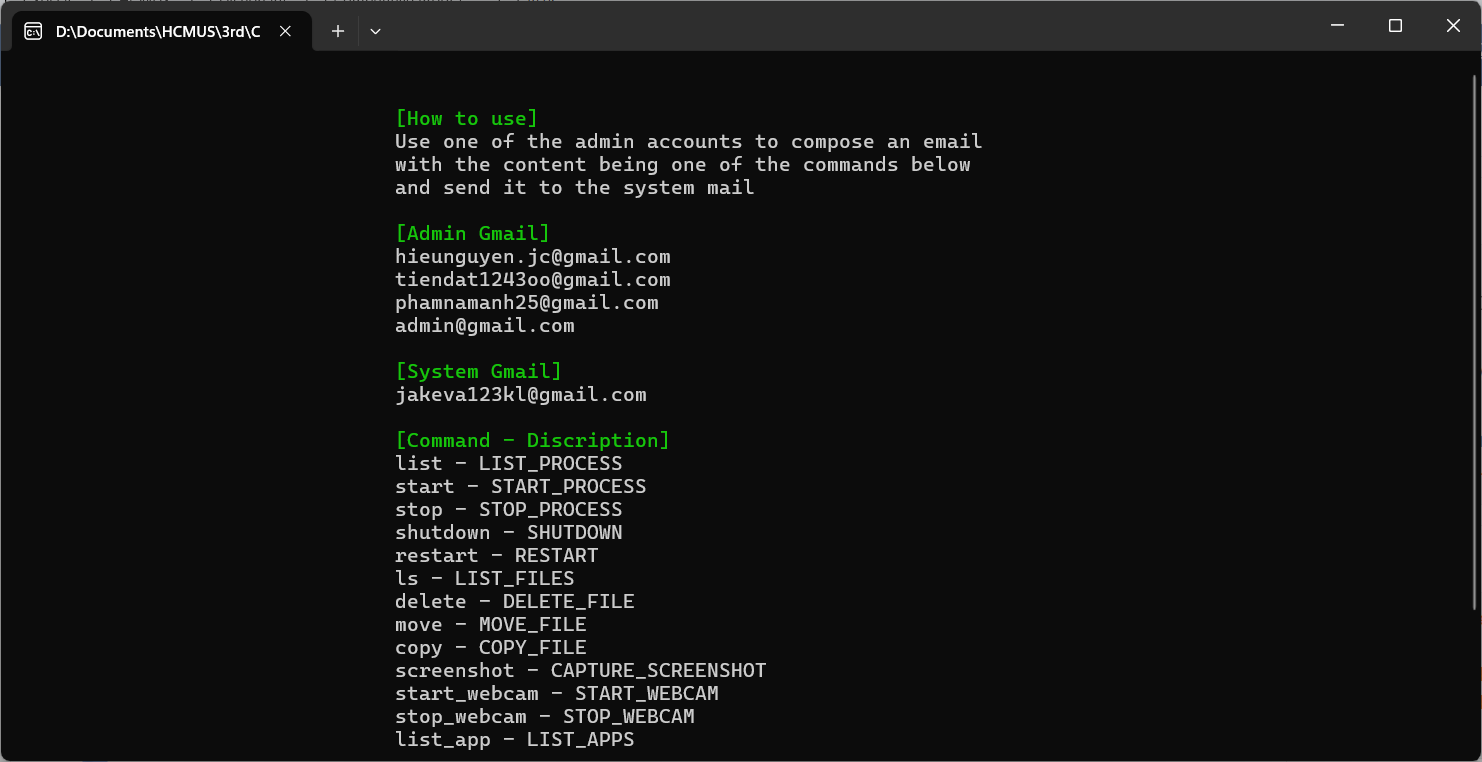
\includegraphics[width=0.7\textwidth]{img/instruction.png}
    \caption{Hướng dẫn sử dụng và các lệnh điều khiển}
\end{figure}

\subsubsection{Server}

Giao diện của server được viết trực tiếp trong hàm \texttt{void main()} hiển thị thông tin về server như IP, tình trạng kết nối với client, và các lệnh điều khiển, dưới đây là hình minh họa cho giao diện của server:

\begin{figure}[H]
    \centering
    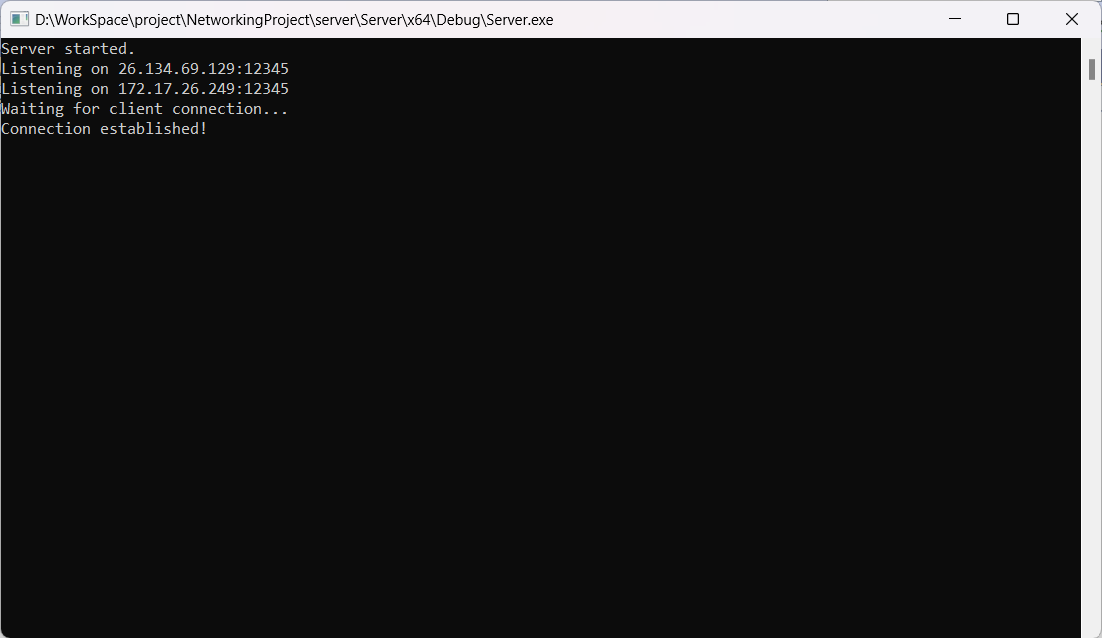
\includegraphics[width=0.7\textwidth]{img/server.png}
    \caption{Giao diện của server}
\end{figure}